\documentclass[tikz]{standalone}
\usepackage[black]{causets}
\usetikzlibrary{fit,shapes.geometric}
% Set colours and style:
\colorlet{future colour}{green!50!black}
\colorlet{past colour}{yellow!50!orange!80!black}
\colorlet{anywhere colour}{red!80!black}
\tikzset{prob arrow/.style={line width=1.5pt}}
% Define some helper functions:
\def\defCevents#1#2#3{\xdef\Ea{#1}\xdef\Eb{#2}\xdef\Ec{#3}}
\def\defDevents#1#2#3#4{\expandafter\defCevents#1#2#3\xdef\Ed{#4}}
\newcommand*{\semiopaque}[1]{% Adds a transparency group.
\begin{scope}[transparency group, opacity=0.5]
	#1
\end{scope}
}
\newcommand*{\drawprobarrow}[4][]{% Draws a (probability) arrow.
\draw[prob arrow] (#2) -- node[sloped, midway, below, #1] {$#3$} (#4);
}
\newcommand{\drawlegendsymbol}{% Draws the symbol for a legend entry.
\draw[prob arrow] (0,0) -- +(10pt, 6pt);
}
\newcommand{\legendsymbol}[1]{% Creates the legend symbol.
\begin{tikzpicture}
	\ifnum#1=0
		\drawlegendsymbol
	\else
		\semiopaque{\drawlegendsymbol}
	\fi
\end{tikzpicture}
}
\begin{document}
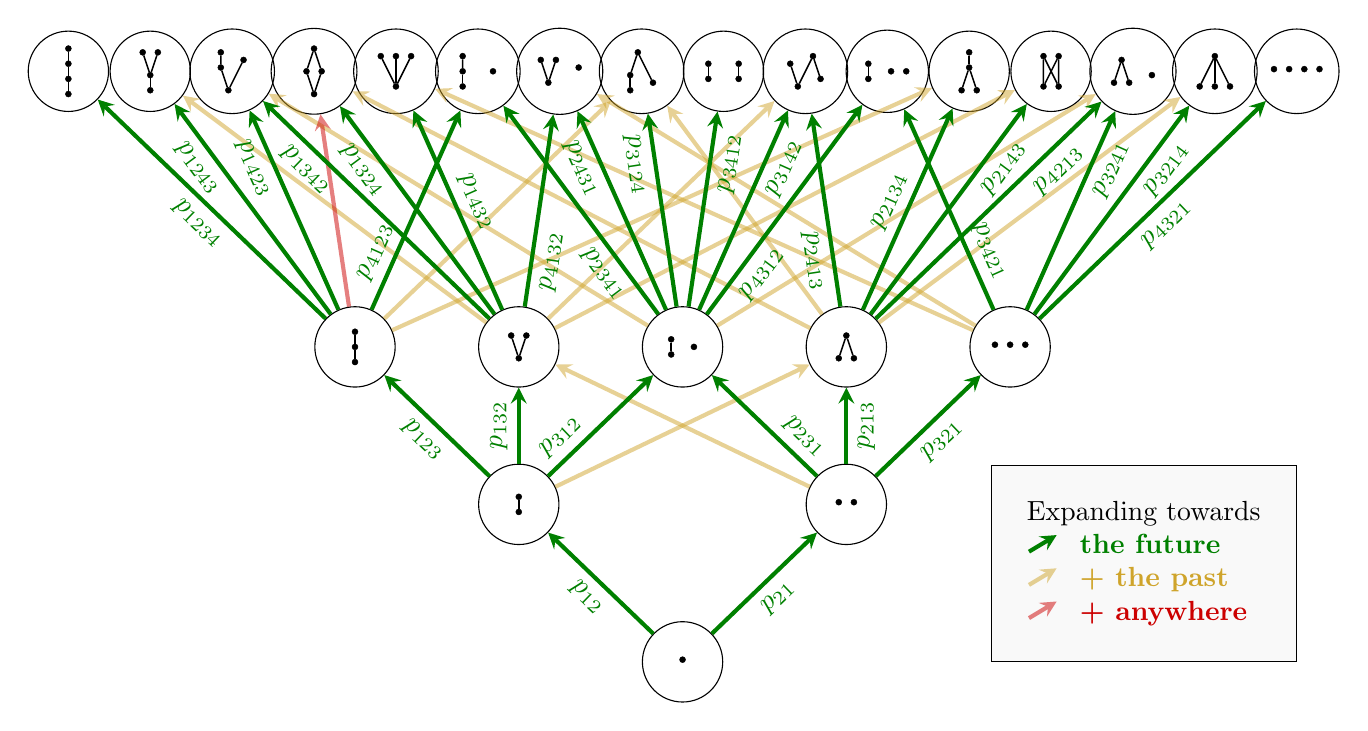
\begin{tikzpicture}[-stealth]
	\def\ystep{2.0cm}
	\def\xstep{0.52cm}
	% Create nodes of all causets with 1 to 4 events:
	\begin{scope}[nodes={draw, thin, circle, minimum size=1.02cm}]
		\node (C1) at ( 0,  0) {\pcauset{1}};
		\node (C12) at (-4*\xstep,  1*\ystep) {\pcauset{1,2}};
		\node (C21) at ( 4*\xstep,  1*\ystep) {\pcauset{2,1}};
		\foreach \perm [count=\i from 0] in {123, 132, 312, 213, 321}{%
			\expandafter\defCevents\perm
			\node (C\perm) at (4*\i*\xstep-8*\xstep, 2*\ystep) {\pcauset{\Ea,\Eb,\Ec}};
		}
		\foreach \perm [count=\i from 0] in {1234, 1243, 1423, 1324, 1432, 4123, 4132, 3124, 3412, 3142, 4312, 2134, 2143, 4213, 3214, 4321}{%
			\expandafter\defDevents\perm
			\node (C\perm) at (2*\i*\xstep-15*\xstep, 3.75*\ystep) {\pcauset{\Ea,\Eb,\Ec,\Ed}};
		}
	\end{scope}
	% Add graph edges for expandings ...
	% ... to the past (additionally):
	\begin{scope}[past colour]
		\foreach \perma/\permb in {12/213, 123/3124, 123/2134, 132/1243, 132/3142, 132/2143, 312/1423, 312/4213, 213/1324, 213/3124, 213/3214, 321/1432, 321/4132, 21/132}
			\semiopaque{\drawprobarrow{C\perma}{}{C\permb}};
	\end{scope}
	% ... to anywhere (additionally, further):
	\begin{scope}[anywhere colour]
		\semiopaque{\drawprobarrow{C123}{}{C1324}};
	\end{scope}
	% ... to the future:
	\begin{scope}[prob arrow, future colour]
		\drawprobarrow{C1}{p_{12}}{C12}
		\drawprobarrow{C12}{p_{123}}{C123}
		\drawprobarrow{C123}{p_{1234}}{C1234}
		\drawprobarrow[near end]{C123}{p_{1243}}{C1243}
		\drawprobarrow[near end]{C123}{p_{1423}}{C1423}
		\drawprobarrow[near start, above]{C123}{p_{4123}}{C4123}
		\drawprobarrow[above]{C12}{p_{132}}{C132}
		\drawprobarrow[near end]{C132}{p_{1342}}{C1423}
		\drawprobarrow[near end]{C132}{p_{1324}}{C1324}
		\drawprobarrow[midway, above]{C132}{p_{1432}}{C1432}
		\drawprobarrow[near start]{C132}{p_{4132}}{C4132}
		\drawprobarrow[near start, above]{C12}{p_{312}}{C312}
		\drawprobarrow[near end]{C312}{p_{3124}}{C3124}
		\drawprobarrow[near end]{C312}{p_{3412}}{C3412}
		\drawprobarrow[near end]{C312}{p_{3142}}{C3142}
		\drawprobarrow[near start]{C312}{p_{4312}}{C4312}
		\drawprobarrow{C1}{p_{21}}{C21}
		\drawprobarrow[near start, above]{C21}{p_{231}}{C312}
		\drawprobarrow[near start]{C312}{p_{2341}}{C4123}
		\drawprobarrow[near end]{C312}{p_{2431}}{C4132}
		\drawprobarrow{C21}{p_{213}}{C213}
		\drawprobarrow[above]{C213}{p_{2134}}{C2134}
		\drawprobarrow[near start]{C213}{p_{2413}}{C3142}
		\drawprobarrow[near end]{C213}{p_{2143}}{C2143}
		\drawprobarrow[near end]{C213}{p_{4213}}{C4213}
		\drawprobarrow{C21}{p_{321}}{C321}
		\drawprobarrow[near start, above]{C321}{p_{3421}}{C4312}
		\drawprobarrow[near end]{C321}{p_{3241}}{C4213}
		\drawprobarrow[near end]{C321}{p_{3214}}{C3214}
		\drawprobarrow{C321}{p_{4321}}{C4321}
	\end{scope}
	% Add legend:
	\node[above left, align=left, draw, inner sep=3ex, fill=gray!05]
		at (15*\xstep, 0)
		{Expanding towards\\
		 \bfseries\color{future colour}\legendsymbol{0}\ the future\\
		 \bfseries\color{past colour}\legendsymbol{1}\ + the past\\
		 \bfseries\color{anywhere colour}\legendsymbol{1}\ + anywhere};
\end{tikzpicture}
\end{document}
